%\documentclass[landscape]{sciposter}
\documentclass[portrait]{sciposter}

\newcommand{\todo}[1]{ \fbox{{\bf TODO:} \color{red} #1}}
\usepackage{amsmath}
\usepackage{amssymb}
%\usepackage{epsfig}
%\usepackage{fancybullets}
\usepackage{multicol}
\usepackage{rotating}
\usepackage{tikz,pgfplots}
\usepackage{siunitx}
\usepackage{wrapfig}


\sisetup{output-exponent-marker=\textsc{e},
bracket-negative-numbers,open-bracket={\text{-}}, close-bracket={}}

\newtheorem{Def}{Definition}

\newcommand{\Div}{\mathrm{Div}_{\gamma}}
\newcommand{\ee}{\mathbf{e}}
\newcommand{\esigma}{e_{\sigma}}
\newcommand{\exx}{\mathbf{e}_{\xx}}
\newcommand{\grad}{\triangledown}
\newcommand{\ff}{\mathbf{f}}
\newcommand{\rr}{\mathbf{r}}
\newcommand{\sdc}{{\,\mathrm{SDC}}}
\newcommand{\ssigma}{\boldsymbol{\sigma}}
\newcommand{\tsigma}{\tilde{\sigma}}
\newcommand{\txx}{\tilde{\xx}}
\newcommand{\uu}{\mathbf{u}}
\newcommand{\xx}{\mathbf{x}}
\newcommand{\yy}{\mathbf{y}}
\newcommand{\BB}{\mathcal{B}}
\renewcommand{\SS}{\mathcal{S}}
\newcommand{\TT}{\mathcal{T}}

%\usetikzlibrary{spy,backgrounds,decorations}
%\usetikzlibrary{spy}

%\usepgfplotslibrary{external}
%\tikzexternalize

\definecolor{SectionCol}{RGB}{120,47,64}
% background color of boxes

\definecolor{BoxCol}{RGB}{206,184,136}
% uncomment for dark blue \section text 

\title{\textcolor{SectionCol}{Automatic Portrait Segmentation of Cats and Dogs}}

% Note: only give author names, not institute
\author{Kevin Mueller, Gordon Erlebacher, Jeremy Quinto*, Iman Dhillon*}
 
% insert correct institute name
\institute{Department of Scientific Computing, Florida State University \\
*NewSciLabs, Tallahassee FL}
% \institute{Department of Mathematics}
% \institute{New Sci}

%\email{quaife@ices.utexas.edu}  % shows author email address below institute

%\date is unused by the current \maketitle


% Logos
\leftlogo[1.1]{DSC-garnet-trans-bg-poster.png}
\rightlogo[1.3]{new_sci_logo.png}

% The following commands can be used to alter the default logo settings
%\leftlogo[0.9]{logoWenI}{  % defines logo to left of title (with scale factor)
%\rightlogo[0.52]{RuGlogo}  % same but on right

% NOTE: This will require presence of files logoWenI.eps and RuGlogo.eps, 
% or other supported format in the current directory  
%%%%%%%%%%%%%%%%%%%%%%%%%%%%%%%%%%%%%%%%%%%%%%%%%%%%%%%%%%%%%%%%%%%%%%%%%%%%%%%%
%%% Begin of Document

\vspace{-100 pt}

\begin{document}

%define conference poster is presented at (appears as footer)

%\conference{Mathematical Foundations for Fast Multi-resolution
%Interactions \& Large Data Analysis}

%\LEFTSIDEfootlogo  
% Uncomment to put footer logo on left side, and 
% conference name on right side of footer

% Some examples of caption control (remove % to check result)

%\renewcommand{\algorithmname}{Algoritme} % for Dutch
%\renewcommand{\mastercapstartstyle}[1]{\textit{\textbf{#1}}}
%\renewcommand{\algcapstartstyle}[1]{\textsc{\textbf{#1}}}
%\renewcommand{\algcapbodystyle}{\bfseries}
%\renewcommand{\thealgorithm}{\Roman{algorithm}}

\maketitle

%%% Begin of Multicols-Enviroment
\begin{multicols}{2}

%%% Abstract
\begin{abstract}
With the ever-growing amount of image data available on the internet, there is an increasing need to develop algorithms that can automatically detect regions of interest (ROI) in images. Currently, almost all approaches for solving this task rely on difficult-to-create supervised datasets that require labels for individual pixels. Here we present an end-to-end framework for automatically cropping images of cats, dogs, and humans by utilizing post-manipulated images prepared by graphic designers. We accomplish this task by first applying an image reconciliation technique that creates pixel masks from the post-manipulated images and then implement a machine learning technique that learns the masks from the original images by utilizing Deep Gaze II, a deep learning model for creating saliency maps trained on human eye-tracking data, as pre-training for finding likely ROIs. 
\end{abstract} 


%%%% Introduction
\section*{Introduction}

Image segmentation is a popular problem in machine learning with numerous applications. There are many different approaches for image segmentation, but they can generally be divided into supervised and unsupervised approaches. Supervised approaches use labeled pixels to learn the correct segmented classes, while unsupervised methods make use of local image properties, such as sharp edges, as a way to segment an image. In general, supervised approaches are the most successful. For example, semantic segmentation treats each individual pixel as a label for a set number of classes and learns a mapping (typically with a deep neural network) from the input pixels to the class labels. 
\\ 
\\
Another approach for image segmentation relies on mimicking how humans process images. In particular, various datasets for eye-tracking have been studied as starting points for detecting ROIs. More recently, this research direction has been combined with deep learning to create a power approach for learning saliency maps. Deep Gaze II is one example of this type of network,which works by randomly sampling feature maps from VGG-16 and passing them through a read-out convolutional network. 
\\ 
\\
For this work we consider a retraining of the Deep Gaze II network on a custom dataset for portrait segmentation. Portrait segmentation is abstractly defined as finding the best portrait-like segmentation for a particular image. Typically, it includes background removal and important facial/head features, but may also include parts of the neck and various accessories.

% \begin{minipage}{.2\textwidth}


% \end{minipage}

\section*{Dataset}

\begin{itemize}
    \item The original dataset consists of approximately 40,000 pairs of photos of cats, dogs, humans, and other animals. 
    \item Each pair consists of an original photo and a post-processed image prepared by professional graphic designers to mimic/represent what subjectively makes a good portrait.
    \item In order to simplify the problem, we only consider images of cats and dogs.
    \item The dataset was split into training/test datasets with a 0.2\% train/test split.
\end{itemize}

 %due to the difficulty of finding accurate representations of images that %have all the required invariances.
 
\section*{Image Reconciliation Model}
Since the goal of this project is to automatically extract the crop  from the original image, it is necessary to first reconcile the post-processed image with the original image. However, since the post-processed image typically undergoes significant modification (e.g. as color, rotation, scale, lighting), this can be a formidable task. In order to create lighting and color invariance, we first apply the Laplacian as a way to extract the edges of both the post-processed and original image. We then loop through a grid of rotations/scales and calculate auto-correlations by sliding the post-processed image as a kernel across the original image.
\\
\\
Due to the brute force method of looping over a large number of rotation/scale combinations, it is useful to utilize GPUs to quickly perform the convolutions. To accomplish this task, we use pytorch  to create a convolutional layer  (with appropriate padding) with a total number of filters equal to the total number of looped rotations and scales.



\begin{figure}
	\centering
	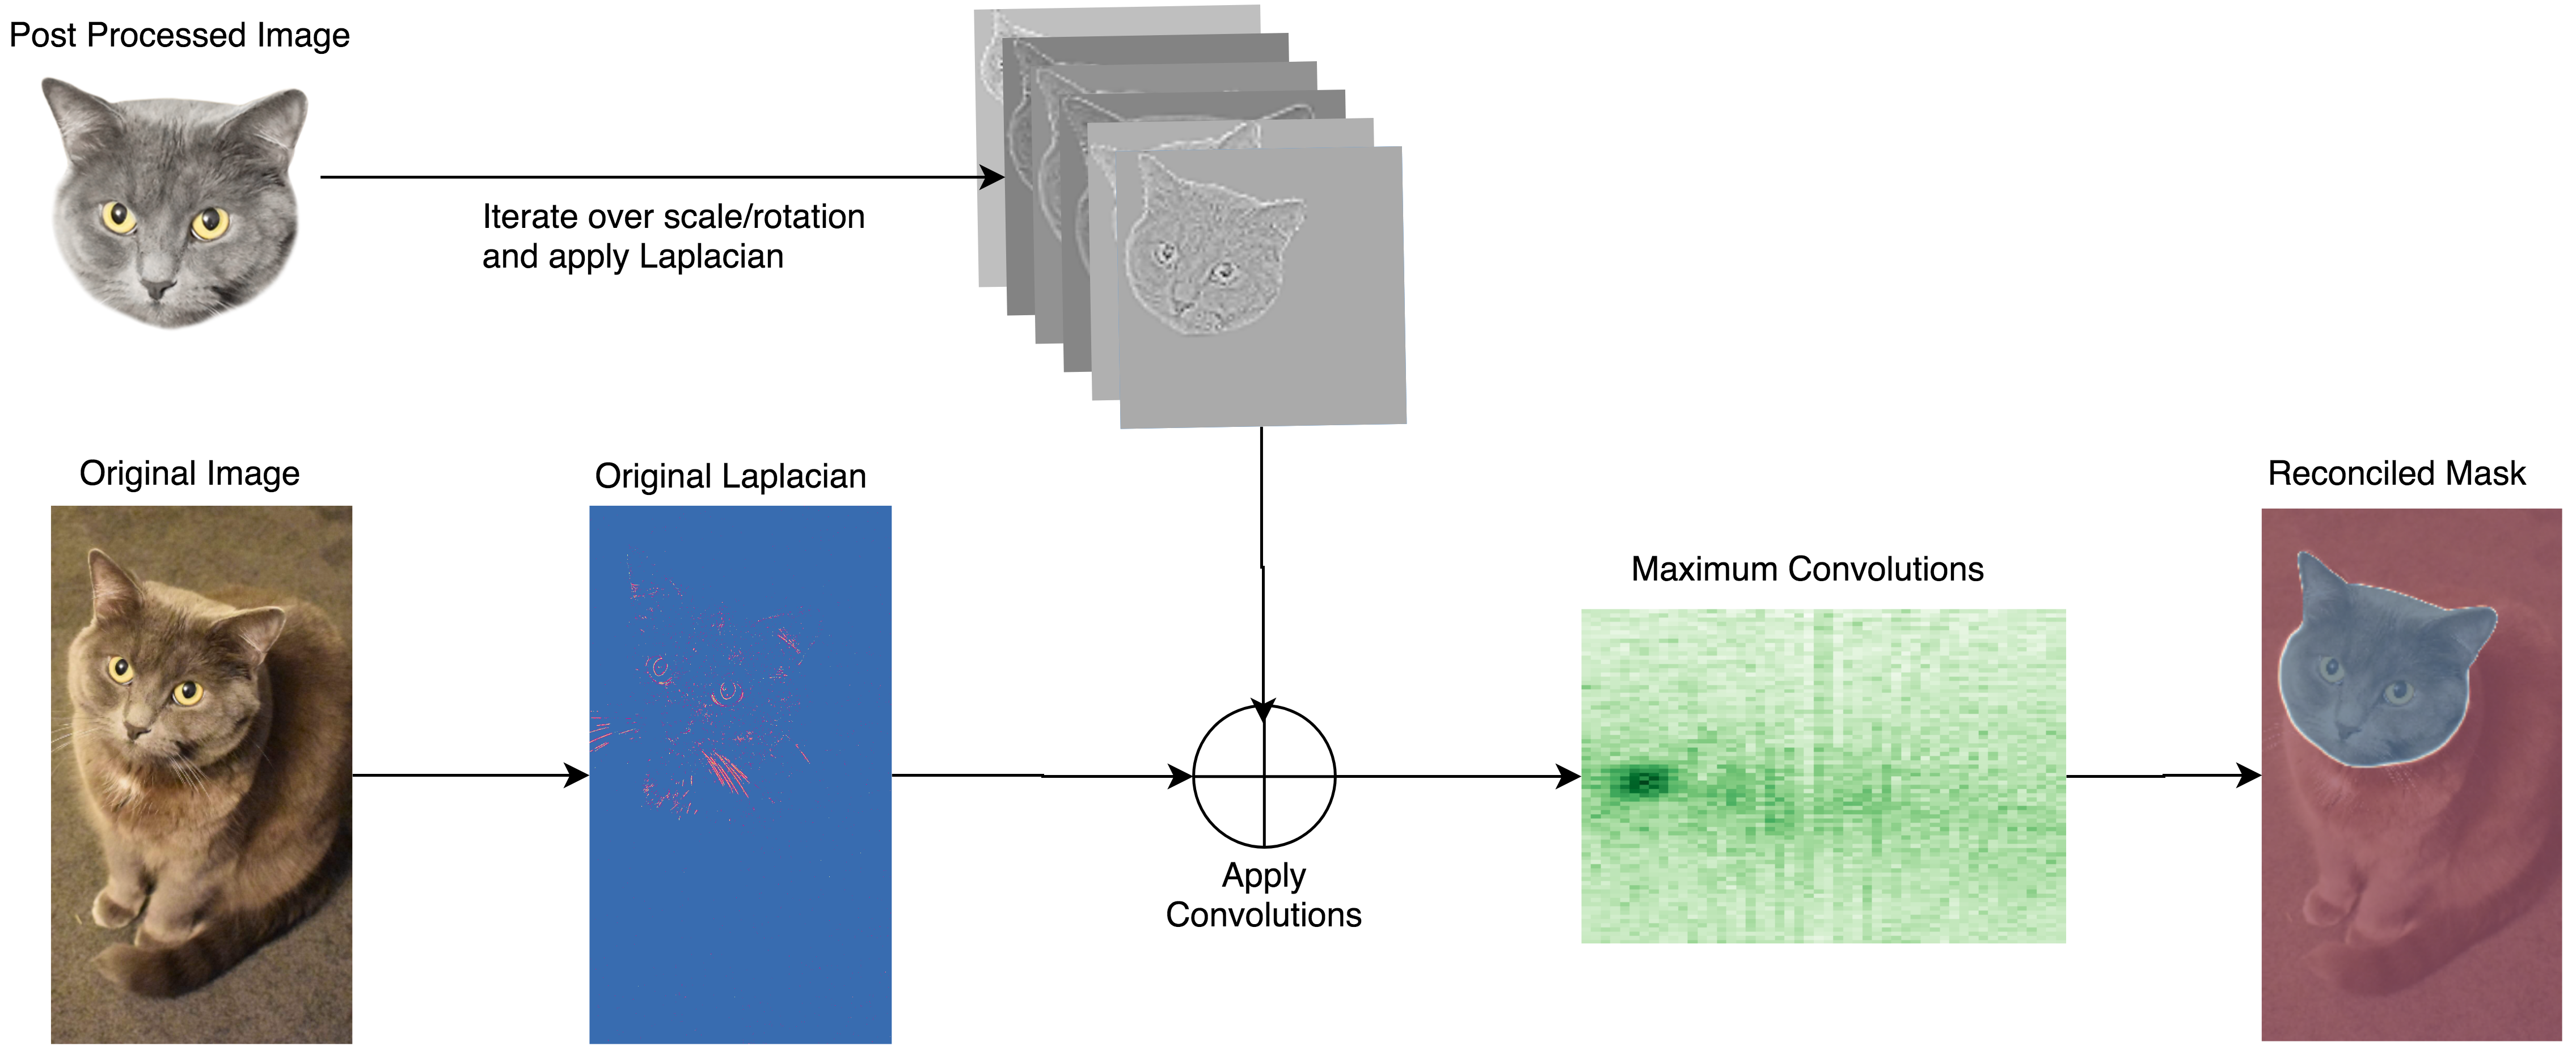
\includegraphics[width=0.9\textwidth]{ImageReconciliation.png}
	\caption{\small The Laplacian is applied to the original image and all scales and rotations of the post-processed image. The resized and rotated images are then convolved with the Laplacian of the original image and the maximum convolution value is calculated. The optimal rotation/scale is found by taking the maximum of the maximum convolutions. Finally, the maximum position of the convolution for the optimal rotation/scale is taken to be the final reconciled mask location.}
\end{figure}

\section*{Automatic Cropping Model}

After the correct crop location in the original image has been found the next step is to apply machine learning to automatically crop the head from the original image. To accomplish this task, we apply transfer learning using the architectures of two other powerful deep-learning architectures:

\begin{itemize}
    \item  \textbf{VGG-16}: A standard deep learning model for image classification. It consists of 5 convolutional blocks, each with 3 to 4 convolutional layers, and makes heavy use of spatial pooling to rapidly increase the receptive field. 

    \item  \textbf{Deep Gaze II}: A network designed to build a probability distribution over pixels from eye-tracking data points. It utilizes VGG-16 as a pretrained network and appends a read-out network that consists of convolutional blocks that take sampled VGG-16 feature maps as input.
\end{itemize}

We create our new loss function by maximizing the log-likelihood of the dataset as

$$ \mathcal{L} = \frac{1}{N} \sum_i \log{p(x_i,y_i,I_i)}  $$,

for the pixel locations $(x_i,y_i)$ in the image $I_i$. This equivalent to minimizing the cross-entropy 

$$ H(p(x,y),q(x,y)) = - \sum_i \log{\left(p(x_i,y_i)\right)} q(x_i,y_i)  $$ 

between the pixel locations $(x_i,y_i)$ between the (true) mask $q_i$ and prediction probabilities $p_i$. 
Finally, since our output from the network is a log-probability we convert the output to a binary mask by applying a simple thresholding function.


\begin{figure}
	\centering
	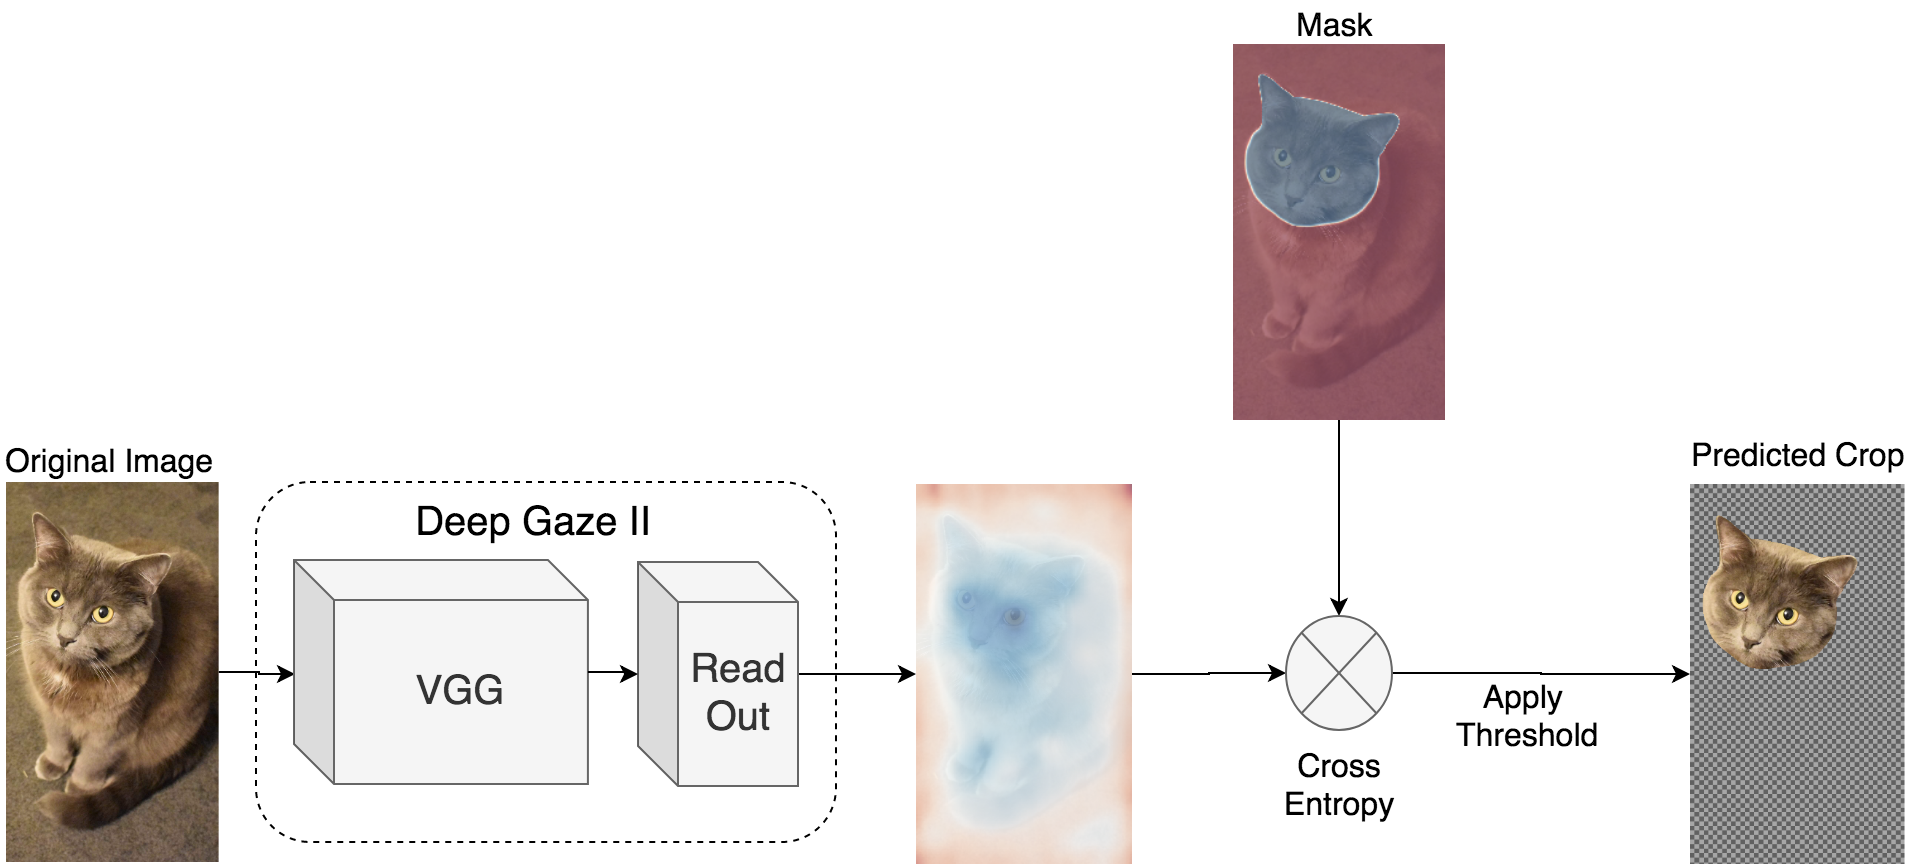
\includegraphics[width=0.9\textwidth]{CropPrediction.png}
	\caption{\small The original image is first fed into the Deep Gaze II network which returns a log probability of the original image from its prior training. The mask is then used to further guide the network to the area of interest of the correctly cropped head. Finally, a threshold is applied to create a binary mask for the original image}
\end{figure}

% \begin{figure}
% \centering
% \includegraphics[width=\textwidth]{POSTERFIG2.pdf}
% \caption{\small Vesicle moving through a constricted geometry with varying Hamaker constants. For larger Hamaker constants, the vesicle has a higher bending energy so that the adhesive energy can be further reduced. In these simulations $\delta = 0.1$, there are $256$ points on the vesicle surface, $512$ points on the substrate, the relative tolerance for area and length are $0.1$, $\kappa_b = 0.1$, the reduced area is $0.65$, and the vesicle is scaled to be $2.6$ times the size of the constriction of $\Omega$.} 
% \end{figure}

% \begin{figure}
% 	\centering
% \includegraphics[width=\textwidth]{fig2.pdf}
% \caption{\small Minimum distance between the vesicle and the substrate as a function of time. As the Hamaker constant increases, the vesicle remains close to the wall for a longer period of time after passing through the constriction. The images of the vesicle configuration correspond to the simulation with Hamaker constant $\mathcal{H} = 0.1$. The dashed line is at $\delta = 0.1$.}
% \end{figure}


\section*{Results}
  We use the Deep Gaze II readout network's pre-training but further modify the weights at training. In contrast, the VGG-16 weights are fixed and not further trained. Additionally, we down scale all image/mask pairs to fit into a fixed-size input of 800 x 800 and pad the unused pixels with zeros. 


\begin{figure}
\centering
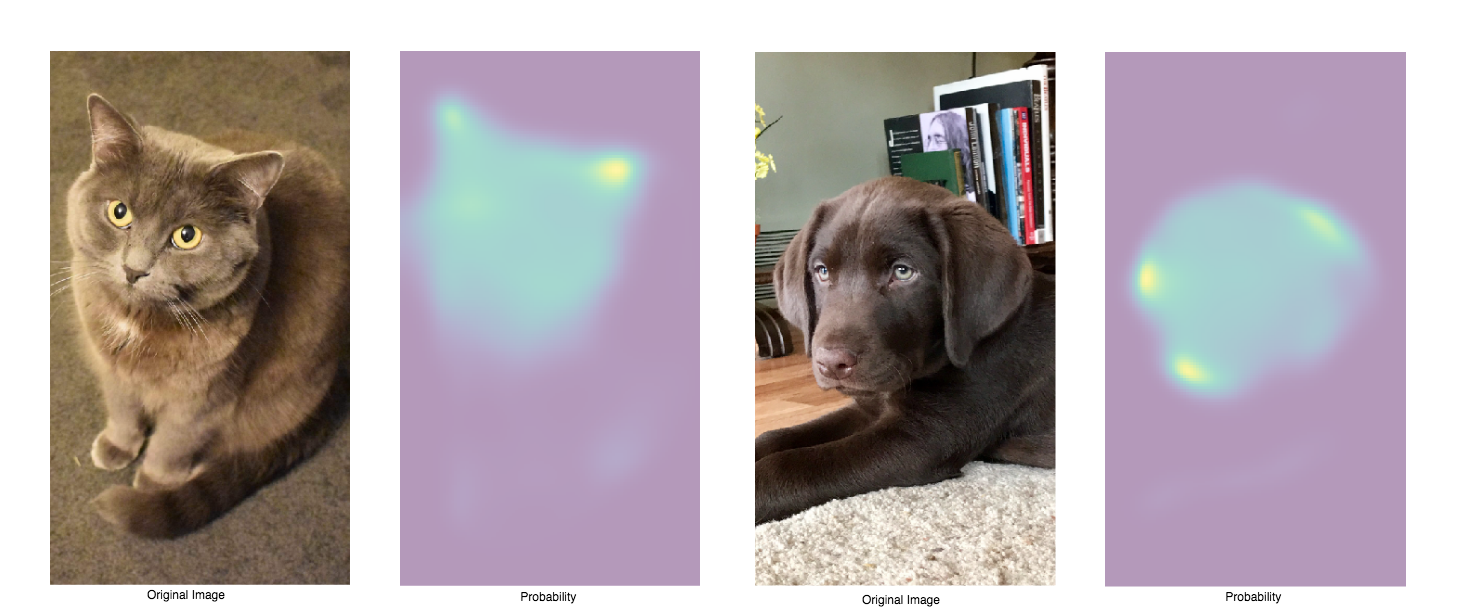
\includegraphics[width=\textwidth]{all_results_cropped_bot.png}
\caption{\small Examples of original images and their predicted probabilities from the validation set.}
\end{figure}

% \begin{figure}
% \centering
% 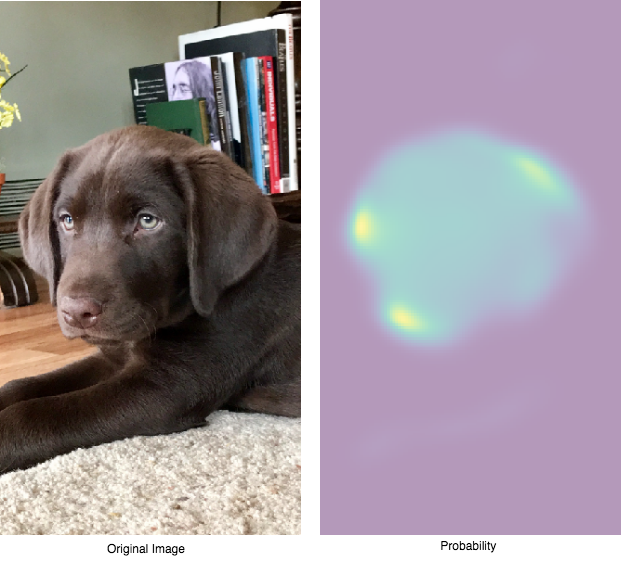
\includegraphics[width=\textwidth]{Dog Results.png}
% \caption{\small Hello} 
% \end{figure}




%%%% Discussion
\section*{Discussion}
\begin{itemize}
	\item Results are promising for training on sets of dogs and cats jointly
	\item Using saliency map/eye-tracking data as pre-training could be useful for binary classification image segmentation tasks.
	\item Transfer learning is a powerful technique for training models on less data.
	\item The threshold is currently set by hand but could be integrated as part of the learning process.
	\item The probability output of the image-cropping model provides a substantial amount of information, which could be applied by the image reconciliation task to approximate the optimal scale/rotation to reduce the total number of required convolutions.
\end{itemize}


\bibliographystyle{plain}
\begin{thebibliography}{1}

\bibitem{qua:Kumm}
Matthias Kummerer, Thomas S. A. Wallis and Matthias Bethge.
\newblock {DeepGaze II: Reading fixations from deep features trained on object recognition.}
\newblock {\em arxiv}, 1610.01563, 2016.

\bibitem{Blo:Mich}
Karen Simonyan, Michael J. and Andrew Zisserman.
\newblock{Very Deep Convolutional Networks for Large Scale Image Recognition}
\newblock {\em arxiv}, 1610.01563, 2016.



\end{thebibliography}


\end{multicols}

\end{document}

